\section{Release Maintainence}

Managing Releases
\newline
Releases for a project can easily be added, deleted and updated using Murcs. To begin select 'Releases' in the Display Choice picker (circled in Figure 23)

\begin{figure}[H]
\centering
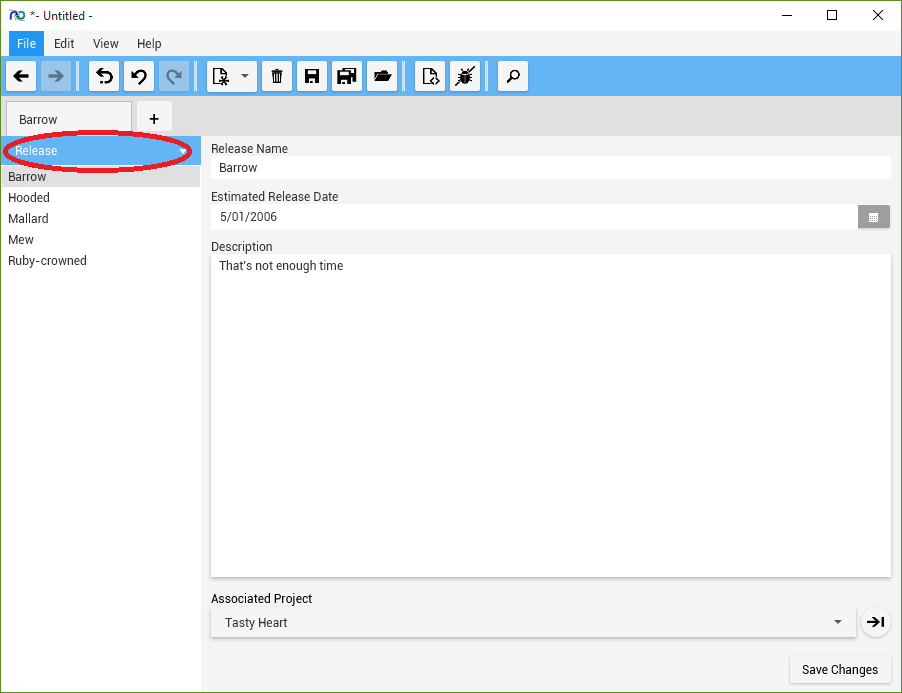
\includegraphics[width=\textwidth]{images/screenshots/releases1.PNG}
\caption{The Display Choice Picker}
\label{fig:new_project}
\end{figure}

Creating Releases
\newline
Now, to add a new release, simply press new button (circled in Figure 24) on the toolbar and you will be presented with a form for creating a new release. Note that new button is context sensitive and the type of element you create will depend on what section of the application you are in. Pressing the little down arrow on the right hand side of it will open a list of all the items you can create.

\begin{figure}[H]
\centering
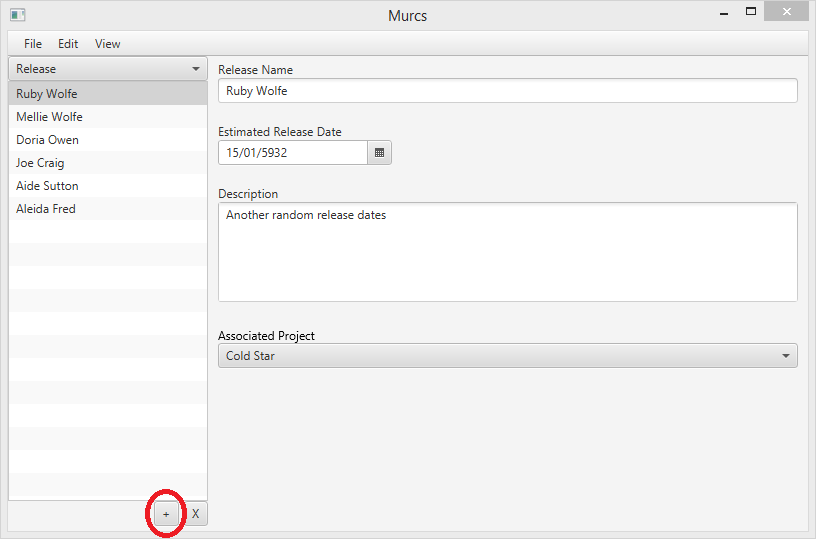
\includegraphics[width=\textwidth]{images/screenshots/releases2.PNG}
\caption{The Add Button}
\label{fig:new_project}
\end{figure}

You will then be presented with a form for creating a new release like the one shown in Figure 25:

\begin{figure}[H]
\centering
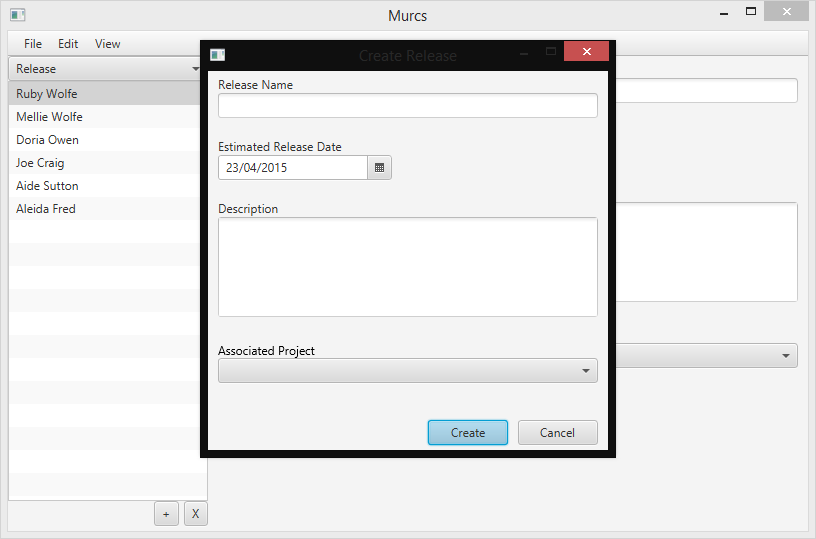
\includegraphics[width=\textwidth]{images/screenshots/releases3.PNG}
\caption{Creating a new release}
\label{fig:new_project}
\end{figure}

Constraints
\newline
There are several constraints you need to take into account when creating a release. Firstly, a release must be given a unique name within the platform, so it can quickly and easily be identified within the application and secondly, a release must have an associated project. If a constraint is not met then a small message will be shown explaining the problem.

Editing Releases
\newline
Any release can be edited by selecting it from the Display List. Upon selection, the form on the right will be populated with all the fields that you can edit. Any changes you make will be automatically saved.

\begin{figure}[H]
\centering
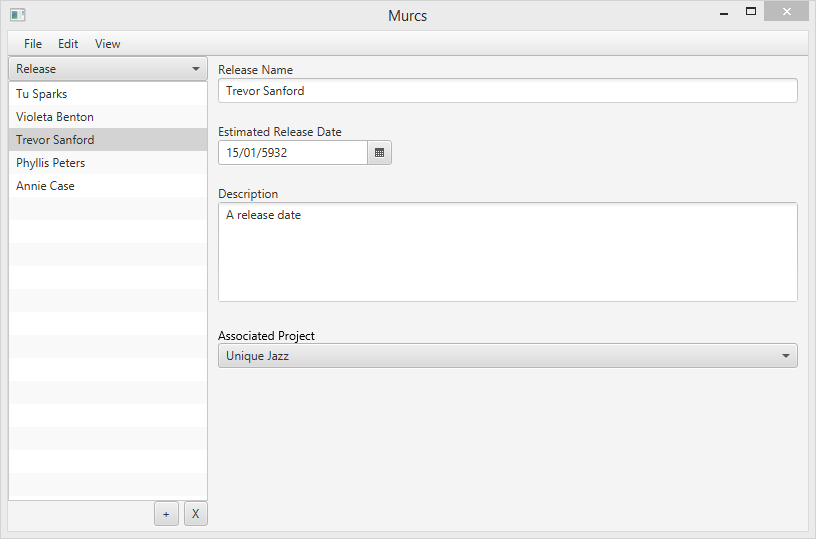
\includegraphics[width=\textwidth]{images/screenshots/releases4.PNG}
\caption{Editing the Release Named 'Barrow'}
\label{fig:new_project}
\end{figure}

Deleting Releases
\newline
Releases can be deleted in the same manner as any other element, by clicking the delete button on the toolbar. For a more in depth explanation, see the element deletion section of this guide
